\section{基本知識}
    \subsection{什麼是樹}
    樹是一個連通圖,裡面沒有環,也沒有自己連自己的邊。因此,
    樹如果有$n$個節點,就會有$n-1$個邊。移除任何一個邊都會
    導致他變成兩棵樹,新增任何邊都會導致出現一個環。

    樹上的任意兩個點擁有唯一路徑,因此我們有機會在$O(\log{(n)})$
    的時間內求出路徑長。也可以發展屬於樹的高效演算法。

    只有連接到一個邊的節點我們稱為葉節點。如果有根(root),則無論
    根連接幾個邊我們都稱他為根結點。

    \begin{figure}[h]
        \centering
        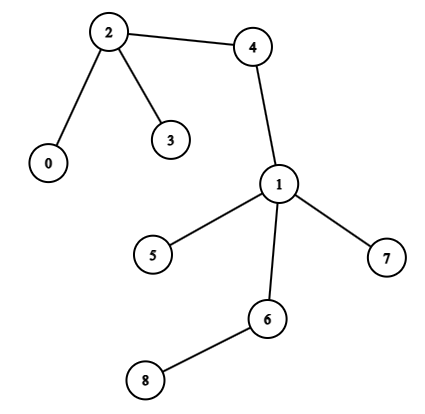
\includegraphics[width=0.8\textwidth]{../Images/Tree.png}
        \caption{樹示意圖}
    \end{figure}

    \subsection{資料儲存}
    通常來說,樹的儲存與圖相同,主要以鄰接串列儲存,不過
    由於樹的特性,如果是有根樹的話,我們可以使用一個陣列儲存,
    每個節點將儲存他的parent node。而如果邊有權重,則可以另外定義edge。

\begin{lstlisting}[caption=樹的儲存]
const int N=100010;
struct edge{
    int to,dis;// 或 w,c etc.
};

vector<int> g[N];
vector<edge> g[N];
int p[N];// 存放 parent
\end{lstlisting}

    \subsection{樹的遍歷}
    樹上可以使用兩種搜索,大致跟圖相同,分別是深度優先搜索(DFS)
    與廣度優先搜索(BFS)。

    深度優先搜索與廣度優先搜索都會定根,就是決定root是誰,如果題目沒有指定,
    也可以直接選擇0或1。

    以下都將以無權重圖演示。

\begin{lstlisting}[caption=DFS in Tree]
void dfs(int now,int parent){
    for(auto next:g[now]) if(next!=parent){
        dfs(next,now);
    }
}
\end{lstlisting}

\begin{lstlisting}[caption=BFS in Tree]
bool isv[N];
void bfs(int root){
    queue<int> nodes;
    nodes.push(root);
    while(!nodes.empty()){// 也可以使用 nodes.size()
        int now=nodes.front();
        nodes.pop();
        // do something below

        for(auto next:g[now]) if(!isv[next]){
            isv[next]=true;
            nodes.push(next);
        }
    }
}
\end{lstlisting}

    在樹上,我們幾乎都使用DFS,因為兩者都會跑完所有節點,
    而DFS的碼量較小,簡單說就是偷懶。

    \subsection{範例與練習}

    \example 洛谷P5908 貓貓和企鵝

    \textbf{題目敘述}

    王國裡有 $n$ 個居住區,它們之間有 $n-1$ 條道路相連,並且保證從每個居住區出發都可以到達任何一個居住區,並且每條道路的長度都為 $1$。

    除了 $1$ 號居住區外,每個居住區住著一隻小企鵝,有一天一隻貓貓從 $1$ 號居住區出發,想要去拜訪一些小企鵝。可是貓貓非常懶,它只願意去距離它在 $d$ 以內的小企鵝們。

    貓貓非常懶,因此希望你告訴他,他可以拜訪多少隻小企鵝。

    \textbf{輸入說明}

    第一行兩個整數 $n, d$,意義如題所述。

    第二行開始,共 $n - 1$ 行,每行兩個整數 $u, v$,表示居民區 $u$ 和 $v$ 之間存在道路。
    
    \textbf{輸出說明}

    一行一個整數,表示貓貓可以拜訪多少隻小企鵝。

    \textbf{範例測試}

    \begin{tabular}{|m{7cm}|m{7cm}|}
        \hline
        範例輸入 1 & 範例輸出 1 \\
        \hline
        \verb|5 1| & \verb|2| \\
        \verb|1 2| & \\
        \verb|1 3| & \\
        \verb|2 4| & \\
        \verb|3 5| & \\
        \hline
    \end{tabular}

    我們可以在dfs函式內加上一個參數dis,表示至今走過的距離。

\begin{lstlisting}[caption=貓貓和企鵝題解]
int d;
int dfs(int now,int parent,int dis=0){
    if(dis>d) return 0;

    int ret=0;
    if(now!=1) ret=1;

    for(auto next:g[now]) if(next!=parent){
        ret+=dfs(next,now,dis+1);
    }

    return ret;
}

int main(){
    // input
    dfs(1,1,0);
}
\end{lstlisting}

    \problem CF 1676 G White-Black Balanced Subtrees

    \textbf{題目敘述}

    給定一棵由$n$個節點組成的根樹,節點從$1$到$n$進行編號,
    根節點為$1$。還有一個字符串s表示每個節點的顏色:
    如果$s_i=B$,則節點$i$是黑色,如果$s_i=W$,
    則節點$i$是白色。

    樹的子樹被稱為平衡子樹,如果白色節點的數量等於黑色節點的數量。
    計算平衡子樹的數量。

    樹是一個無環的連通無向圖。根樹是一棵樹中選定的節點,
    該節點被稱為根。在這個問題中,所有樹都有根1。

    該樹由包含$n-1$個數字的父節點數組$a_2,\cdots,a_n$來指定:對於所有$i=2,\cdots,n$,
    $a_i$是編號為$i$的節點的父節點。節點$u$的父節點是一個節點,它是從$u$到根之間的一個簡單路徑上的下一個節點。

    節點u的子樹是所有通過u的節點集合,形成從$u$到根的簡單路徑。
    請注意,一個節點包含在其子樹中,並且根的子樹是整棵樹。

    \textbf{輸入說明}

    輸入的第一行包含一個整數$t(1 \le t \le 10^4)$——測試案例的數量。

    每個測試案例的第一行包含一個整數$n(2 \le n \le 4000)$——樹中的節點數量。

    每個測試案例的第二行包含$n-1$個整數$a_2,\cdots,a_n(1 \le ai <i)$——節點$2,\cdots,n$的父節點。

    每個測試案例的第三行包含一個長度為n的字符串s,由字符B和W組成——樹的顏色。

    保證所有測試案例中$n$的值的總和不超過$2 \times 10^5$。
    
    \textbf{輸出說明}

    對於每個測試案例,輸出一個整數——平衡子樹的數量。

    \textbf{範例測試}

    \begin{tabular}{|m{7cm}|m{7cm}|}
        \hline
        範例輸入 1 & 範例輸出 1 \\
        \hline
        \verb|3|           & \verb|2| \\
        \verb|7|           & \verb|1| \\
        \verb|1 1 2 3 3 5| & \verb|4| \\
        \verb|WBBWWBW| & \\
        \verb|2|  & \\
        \verb|1|  & \\
        \verb|BW| & \\
        \verb|8|  & \\
        \verb|1 2 3 4 5 6 7| & \\
        \verb|BWBWBWBW|      & \\
        \hline
    \end{tabular}

    \problem CF 115 A Party

    \textbf{題目敘述}

    一家公司有 $n$ 名員工,編號從 $1$ 到 $n$。每個員工可能沒有直接的經理,
    或者恰好有一位不同編號的員工作為他的直接經理。
    如果滿足以下條件之一,則員工 $A$ 被稱為員工 $B$ 的上級:

    員工 $A$ 是員工 $B$ 的直接經理。
    員工 $B$ 有一位直接經理員工 $C$,且員工 $A$ 是員工 $C$ 的上級。
    公司不會存在管理循環,即不存在一位員工是其直接經理的上級。

    今天公司將舉辦一個派對。這涉及將所有 $n$ 名員工分為若干組:
    每位員工必須屬於且只能屬於一個組。此外,在任何一個組內,
    不能有兩個員工 $A$ 和 $B$,其中 $A$ 是 $B$ 的上級。

    最少需要形成多少組?

    \textbf{輸入說明}

    第一行包含整數 $n (1 \le n \le 2000)$ — 員工的數量。

    接下來的 $n$ 行包含整數 $p_i (1 \le p_i \le n \; 或 \; p_i = -1)$。
    每個 $p_i$ 表示第 $i$ 名員工的直接經理。
    如果$p_i$ 是 $-1$,表示第 $i$ 名員工沒有直接經理。

    保證不會有員工是自己的直接經理 $(p_i \ne i)$。同時,不會存在管理循環。
    
    \textbf{輸出說明}

    輸出一個整數,表示在派對中將形成的最小群組數量。

    \textbf{範例測試}

    \begin{tabular}{|m{7cm}|m{7cm}|}
        \hline
        範例輸入 1 & 範例輸出 1 \\
        \hline
        \verb|5|  & \verb|3| \\
        \verb|-1| & \\
        \verb|1|  & \\
        \verb|2|  & \\
        \verb|1|  & \\
        \verb|-1| & \\
        \hline
    \end{tabular}

    \begin{tip}
        像這種圖裡面有很多樹的情況我們通常稱為樹林。
    \end{tip}